\documentclass[10pt]{beamer}
\usetheme[
%%% option passed to the outer theme
%    progressstyle=fixedCircCnt,   % fixedCircCnt, movingCircCnt (moving is deault)
  ]{Feather}
  
% If you want to change the colors of the various elements in the theme, edit and uncomment the following lines
\definecolor{grey}{rgb}{0.52, 0.52, 0.51}

% Change the bar colors:
\setbeamercolor{Feather}{fg=grey!20,bg=grey}
% This is the inner theme file of the Feather theme.
% Copyright (c) 2014 by Lilyana Vaskova Vankova <lilqna.v@gmail.com>
%
% This program is free software: you can redistribute it and/or modify
% it under the terms of the GNU General Public License as published by
% the Free Software Foundation, either version 3 of the License, or
% (at your option) any later version.
%
% This program is distributed in the hope that it will be useful,
% but WITHOUT ANY WARRANTY; without even the implied warranty of
% MERCHANTABILITY or FITNESS FOR A PARTICULAR PURPOSE.  See the
% GNU General Public License for more details.
%
% You can find the GNU General Public License at <http://www.gnu.org/licenses/>.

%----------------------------------------------------------------------------------------------------------------------------------

\NeedsTeXFormat{LaTeX2e}
\ProvidesPackage{beamerinnerthemeFeather}[2014/04/08 v1.0.0 The Feather Beamer Theme]

%----------------------------------------------------------------------------------------------------------------------------------

%%%%%%%%%%%%%%%%%%%%%%%%%%%%%%%%%%%%%%%%%%%%%%%%
% Theme options, definitions and templates.
%%%%%%%%%%%%%%%%%%%%%%%%%%%%%%%%%%%%%%%%%%%%%%%%

%----------------------------------------------------------------------------------------------------------------------------------

% beamer specific options

               \mode<presentation> %refers to the first four modes (beamer,handout,second and trans). That is, to all modes except the article mode
{

%----------------------------------------------------------------------------------------------------------------------------------

% title page
%% definitions for fonts of the different elements
  
               \setbeamerfont{institute}{family=\rmfamily, size = \footnotesize}
               \setbeamerfont{title}{family=\rmfamily, size = \huge} 
               \setbeamerfont{subtitle}{family=\rmfamily, size = \Large}
               \setbeamerfont{author}{family=\rmfamily, size = \footnotesize}
               \setbeamerfont{date}{family=\rmfamily, size = \footnotesize}

               \setbeamertemplate{title page}
   {

%% setting the above definitions

        \begin{minipage}[c][\textheight][c]{\textwidth}

                  \centering

                 {\usebeamerfont{institute}\insertinstitute}\vspace*{30pt}

                 {\usebeamerfont{title}\usebeamercolor[fg]{title}\inserttitle}\vspace*{10pt}

                 {\usebeamerfont{subtitle}\usebeamercolor[fg]{subtitle}\insertsubtitle}\vspace*{30pt}

                 {\usebeamerfont{author}\insertauthor}\vspace*{30pt}

                 {\usebeamerfont{date}\insertdate}\vspace*{\baselineskip}

         \end{minipage}
   }
  
%----------------------------------------------------------------------------------------------------------------------------------
  
% final page

                  \defbeamertemplate{final page}{text}[1]
   {
         \begin{minipage}[c][\textheight][c]{\textwidth}
                  \centering
                  #1
         \end{minipage}
   }
                  \newcommand{\finalpage}[1]
   {
                  \setbeamertemplate{final page}[text]{#1}
                  \usebeamertemplate{final page}
   }

%----------------------------------------------------------------------------------------------------------------------------------
  
% add the feather to the background of the titlepage and the final page

                  \newcommand{\1}
   {
                  \setbeamertemplate{background}
      {
                  
\includegraphics[height=\paperheight]{Feathergraphics/1}
                  \tikz[overlay] \fill[fill opacity=0.8,fill=white] (0,0) rectangle (-\paperwidth,\paperheight);
       }
    }

%----------------------------------------------------------------------------------------------------------------------------------
  
% use numbers instead of a picture for the references

                  \setbeamertemplate{bibliography item}[text]

}

\mode<all>
% Change the color of the structural elements:
\setbeamercolor{structure}{fg=grey}

% Change the frame title text color:
%\setbeamercolor{frametitle}{fg=blue}

% Change the normal text color background:
\setbeamercolor{normal text}{fg=black,bg=gray!10}

%-------------------------------------------------------
% INCLUDE PACKAGES
%-------------------------------------------------------

\usepackage[utf8]{inputenc}
\usepackage[ngerman]{babel}
\usepackage[T1]{fontenc}
\usepackage{helvet}
\usepackage{lipsum}
\usepackage{tikz}
\usepackage[export]{adjustbox}

\usetikzlibrary{arrows, arrows.meta, positioning}


%-------------------------------------------------------
% DEFFINING AND REDEFINING COMMANDS
%-------------------------------------------------------

% colored hyperlinks
\newcommand{\chref}[2]{
  \href{#1}{{\usebeamercolor[bg]{Feather}#2}}
}

%-------------------------------------------------------
% INFORMATION IN THE TITLE PAGE
%-------------------------------------------------------

\title[] % [] is optional - is placed on the bottom of the sidebar on every slide
{ % is placed on the title page
      \textbf{Wavelength}
}

\subtitle[$\lambda$-IDE]
{
      \textbf{$\lambda$-IDE}
}

\author[wavelength]
{      Jean-Pierre von der Heydt \\  
	   Muhammet Guemues \\
       Markus Himmel \\
       Marc Huisinga \\
       Philip Klemens \\ 
       Julia Schmid   
}

\institute[]
{
      
  
  %there must be an empty line above this line - otherwise some unwanted space is added between the university and the country (I do not know why;( )
}

\date{11. Januar 2018}

%-------------------------------------------------------
% THE BODY OF THE PRESENTATION
%-------------------------------------------------------

\begin{document}

%-------------------------------------------------------
% THE TITLEPAGE
%-------------------------------------------------------

%{\1 % this is the name of the PDF file for the background
% Mein PDF-Viewer bekommt das nicht hin, das Bild im Hintergrund anzuzeigen
{
%\setbeamertemplate{background canvas}{\tikz[remember picture,overlay]\node[opacity=0.3] at (current page.center) {
\includegraphics[height=\paperheight]{img/Logo.pdf}};}
\begin{frame}[plain]
\maketitle
\end{frame}
}
%}


%\begin{frame}{Content}{}
%\tableofcontents
%\end{frame}

\begin{frame}[plain]
	\begin{center}
	\only<1-2>{\begin{tikzpicture}[every path/.style={thick}]
		\node[rectangle, draw] (app) at (0, 0.5) {App};
		\node[rectangle, draw] (model) at (3, -1) {Model};
		\node[rectangle, draw] (view) at (-3, -1) {View};
		\node[rectangle, draw] (controller) at (0, 2) {Controller};

		\draw[-{open diamond}] (app) -- (view);
		\draw[-{open diamond}] (app) -- (model);
		\draw[-{open diamond}] (app) -- (controller);

		\draw[->] (controller.east) to[bend left=40] (model.north);
		\draw[->,dashed] ([yshift=0.1cm]model.west) to ([yshift=0.1cm]view.east);
		\draw[<-] ([yshift=-0.1cm]model.west) to ([yshift=-0.1cm]view.east);
		\draw[->,dashed] ([xshift=0.1cm]view.north) to[bend left=40] ([yshift=-0.1cm]controller.west);
		\draw[->] ([yshift=0.1cm]controller.west) to[bend right=40] ([xshift=-0.1cm]view.north);
	\end{tikzpicture}}
	\only<2-3>{\vfill\begin{tikzpicture}[every path/.style={thick}]
		\node[rectangle, draw] (app) at (0, 0.5) {App};
		\node[rectangle, draw] (model) at (3, -1) {Model};
		\node[rectangle, draw] (view) at (-3, -1) {View};
		\node[rectangle, draw] (controller) at (0, 2) {Controller};

		\draw[-{open diamond}] (app) -- (view);
		\draw[-{open diamond}] (app) -- (model);
		\draw[-{open diamond}] (app) -- (controller);

		\draw[->,dashed] ([xshift=0.1cm]view.north) to[bend left=40] ([yshift=-0.1cm]controller.west);
		\draw[->] ([yshift=0.1cm]controller.west) to[bend right=40] ([xshift=-0.1cm]view.north);
		\draw[->,dashed] ([xshift=0.1cm]model.north) to[bend right=40] ([yshift=0.1cm]controller.east);
		\draw[->] ([yshift=-0.1cm]controller.east) to[bend left=40] ([xshift=-0.1cm]model.north);
	\end{tikzpicture}}
	\only<3>{\vfill\begin{tikzpicture}[every path/.style={thick}]
		\node[rectangle, draw] (app) at (0, 0) {App};
		\node[rectangle, draw] (model) at (2.5, 0) {Model};
		\node[rectangle, draw] (view) at (-2.5, 0) {View};
		\node[rectangle, draw] (action) at (0, 1.8) {Action};
		\node[rectangle, draw] (update) at (0, -1.8) {Update};

		\draw[-{open diamond}] (app) -- (view);
		\draw[-{open diamond}] (app) -- (model);
		\draw[-{open diamond}] (app) -- (action);
		\draw[-{open diamond}] (app) -- (update);

		\draw[->] (action.east) to[bend left=40] (model.north);
		\draw[->,dashed] (model.south) to[bend left=40] (update.east);
		\draw[->] (update.west) to[bend left=40] (view.south);
		\draw[->,dashed] ([xshift=0.1cm]view.north) to[bend left=40] ([yshift=-0.1cm]action.west);
		\draw[->] ([yshift=0.1cm]action.west) to[bend right=40] ([xshift=-0.1cm]view.north);
	\end{tikzpicture}}
	\end{center}
\end{frame}

\begin{frame}[plain]
	\texttt{model.term} package\vfill

	\begin{columns}
	\begin{column}{0.45\textwidth}
	\begin{tikzpicture}[every path/.style={thick}, every node/.style={minimum height=0.8cm, minimum width=3cm}]
		\node[rectangle, draw] (lt) at (0, 0.5) {LambdaTerm};
		%\node[rectangle, draw] (app) at (-4.5, -2) {Application};
		%\node[rectangle, draw] (free) at (-1.5, -2) {FreeVariable};
		%\node[rectangle, draw] (bound) at (1.5, -2) {BoundVariable};
		%\node[rectangle, draw] (abs) at (4.5, -2) {Abstraction};

		%\draw[-{open triangle 45}] (app) -- +(0, 1) -| (lt);
		%\draw[-{open triangle 45}] (free) -- +(0, 1) -| (lt);
		%\draw[-{open triangle 45}] (bound) -- +(0, 1) -| (lt);
		%\draw[-{open triangle 45}] (abs) -- +(0, 1) -| (lt);

		\uncover<2->{
			\node[rectangle, draw] (app) at (-2, -1.1) {Application};
			\node[rectangle, draw] (abs) at (-2, -2.2) {Abstraction};
			\node[rectangle, draw] (free) at (-2, -3.3) {FreeVariable};
			\node[rectangle, draw] (bound) at (-2, -4.4) {BoundVariable};
			\draw[-{open triangle 45}] (app)  -| (lt);
			\draw[-{open triangle 45}] (free)  -| (lt);
			\draw[-{open triangle 45}] (bound)  -| (lt);
			\draw[-{open triangle 45}] (abs)  -| (lt);

			\draw[{open diamond}-] (app) -- +(-2.2, 0) |- (lt);
			\draw[{open diamond}-] (abs) -- +(-2.2, 0) |- (lt);
		}

		\uncover<3->{
			\node[rectangle, draw] (nt) at (-2, -5.5) {NamedTerm};
			\draw[-{open triangle 45}] (nt) -| (lt);
			\draw[{open diamond}-] (nt) -- +(-2.2, 0) |- (lt);

			\node[rectangle, draw] (pa) at (-2, -6.6) {PartialApplication};
			\draw[-{open triangle 45}] (pa) -| (lt);
			\draw[{open diamond}-] (pa) -- +(-2.2, 0) |- (lt);
		}
	\end{tikzpicture}
	\end{column}
	\begin{column}{0.45\textwidth}
		\begin{center}
		\uncover<4->{
			\begin{tikzpicture}[every path/.style={thick}, node distance=1.8cm]
				\node (top) {\textit{app}};

				\node (a) [below left of=top] {\textit{app}};
				\node (b) [below left of=a] {\texttt{func}};

				\node (v1) [below right of=top] {\texttt{5}};
				\node (v2) [below right of=a] {\texttt{6}};

				\draw (top) -- (a);
				\draw (top) -- (v1);
				\draw (a) -- (b);
				\draw (a) -- (v2);
			\end{tikzpicture}
		}
		\end{center}
	\end{column}
	\end{columns}
\end{frame}

\begin{frame}[plain]
	\texttt{model.term} package
	\begin{center}
	\begin{tikzpicture}[every path/.style={thick}, every node/.style={minimum height=0.8cm}]
		\node[rectangle, draw] (v) at (0, 0) {Visitor<T>};
		\uncover<2->{
		\node[rectangle, draw, minimum width=4.5cm] (na) at (3.5, -1.2) {NameAgnosticVisitor<T>};
		\node[rectangle, draw, minimum width=4.5cm] (tt) at (3.5, -2.4) {TermTransformer};
		\node[rectangle, draw, minimum width=4.5cm] (rn) at (3.5, -3.6) {ResolvedNamesVisitor<T>};

		\node[anchor=west] at (6, -1.2) {\textit{z.B. Reduktionsordnung}};
		\node[anchor=west] at (6, -2.4) {\textit{z.B. $\beta$-Reduktion}};
		\node[anchor=west] at (6, -3.6) {\textit{z.B. User Interface}};

		\draw[-{open triangle 45}] (na) -| (v);
		\draw[-{open triangle 45}] (tt) -| (v);
		\draw[-{open triangle 45}] (rn) -| (v);}
	\end{tikzpicture}
	\end{center}
\end{frame}

\begin{frame}[plain]
	\begin{center}
		\begin{tikzpicture}[every path/.style={thick}]

			\node at (0, -0.1) [anchor=south west] {\texttt{model} package};
			\draw (0, -0.1) -- (11, -0.1) -- (11, -3.6) -- (0, -3.6) -- cycle;

			\draw (0, -1) -- (11, -1);
			\draw (0, -0.9) -- (11, -0.9);

			\node at (5.5, -0.55) {\large ExecutionEngine};


			\uncover<2->{
			\node at (0, -1.4) [anchor=west] {\textit{<<constructor>>} ExecutionEngine(String input, List<Library> libraries)};
			\node[anchor=south west] at (0, -4.5) {\texttt{model.parsing} package};
			\node[draw, rectangle, anchor=north west, minimum height=1cm, minimum width=4cm] (parser) at (0, -4.5) {\large Parser};
			\draw[->] (5.5, -3.6) |- (parser);

			\node[anchor=south east] at (11, -4.5) {\texttt{model.library} package};
			\node[draw, rectangle, anchor=north east, minimum height=1cm, minimum width=4cm] (library) at (11, -4.5) {\large Library};
			\draw[->] (5.5, -3.6) |- (library);}

			\uncover<3->{
			\node at (0, -2.0) [anchor=west] {stepForward(Application redex)};
			\node at (0, -2.6) [anchor=west] {stepForward()};
			\node[anchor=south west] at (0, -6.5) {\texttt{model.reduction} package};
			\node[draw, rectangle, anchor=north west, minimum height=1cm, minimum width=4cm] (ro) at (0, -6.5) {\large ReductionOrder};
			\draw[->] (5.5, -3.6) |- (ro);}

			\uncover<4->{
			\node at (0, -3.2) [anchor=west] {stepBackward()};
			\node[anchor=south east] at (11, -6.5) {\texttt{model.output} package};
			\node[draw, rectangle, anchor=north east, minimum height=1cm, minimum width=4cm] (os) at (11, -6.5) {\large OutputSize};
			\draw[->] (5.5, -3.6) |- (os);}

		\end{tikzpicture}
	\end{center}
\end{frame}

\begin{frame}[plain]
	\begin{align*}
		\text{\texttt{view.execution.Executor}} &\to \text{\texttt{model.ExecutionEngine}}\\
		\text{\texttt{view.update.*}} &\to \text{\texttt{model.term.*}}\\
		\text{\texttt{view.App, view.action.*}} &\to
		\begin{cases}\text{\texttt{model.library.*}}\\
		\text{\texttt{model.output.*}}\\
		\text{\texttt{model.reduction.*}}
		\end{cases}
	\end{align*}
\end{frame}

\begin{frame}[plain]
	\begin{center}
		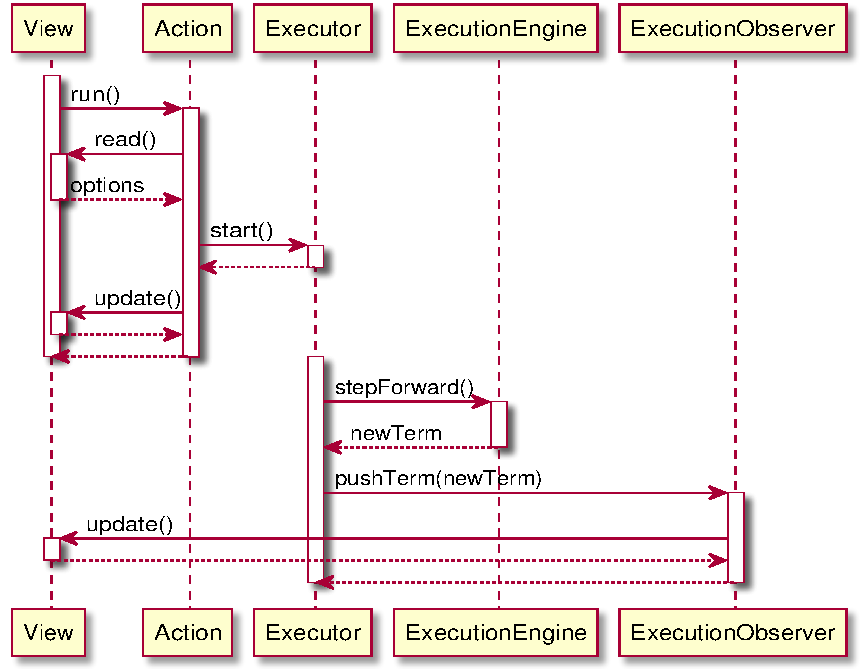
\includegraphics[max size={\textwidth}{\textheight}]{img/exec.pdf}
	\end{center}
\end{frame}

\end{document}
